\documentclass[a4paper,12pt,twoside]{article}

\usepackage{ucs}
\usepackage[utf8]{inputenc}
\usepackage[T1]{fontenc}
\usepackage[frenchb]{babel}
\usepackage{lmodern}
\usepackage{geometry}
\usepackage{graphicx}
\usepackage{amsmath,amssymb}
\usepackage{float} 
\usepackage{tabularx}
\usepackage{lastpage}           % numérotation
\usepackage{fancyhdr}           % en-têtes
\usepackage{verbatim}
\usepackage{mathpazo}           % police Palatino
\usepackage{xcolor}
\usepackage{listingsutf8}

% En-têtes
\pagestyle{headings}

\title{Systèmes distribués\\
  Make distribué}
\author{Bruno \textsc{Jurkovski}\and Élisabeth \textsc{Rousset}}

% \newenvironment{changemargin}[2]%
% {\begin{list}{}{%
%       \setlength{\listparindent}{\parindent}%
%       \setlength{\itemindent}{\parindent}%
%       \setlength{\leftmargin}{#1}%
%       \setlength{\rightmargin}{#2}%
%     }\item }%
%   {\end{list}}

\begin{document}

\maketitle
\newpage

\tableofcontents

\listoffigures

\newpage

\section*{Introduction}

Ce projet a pour but de programmer une version distribuée de \emph{GNU
  make}. L'exécutable créé sera désigné dans la suite de ce document
par le nom \emph{dmake}. Ce programme possède les fonctionnalités
suivantes :
\begin{itemize}
\item parsing de makefiles simples pouvant contenir des variables
\item distribution des tâches sur un ensemble de noeuds
\item transfert des fichiers nécessaires à l'exécution des tâches sur
  les noeuds concernés
\item exécution des tâches sur les noeuds
\item rapatriement des fichiers créés ou modifiés
\end{itemize}
L'archive fournie contient l'ensemble du code source compilable, les
fichiers tests ainsi que le benchmark utilisé pour l'étude de performances.

\section{Travail réalisé}

Cette section détaille les choix de conception ainsi que
l'installation et le déploiement de \emph{dmake}.

\subsection{Langage}

\emph{Dmake} est programmé en langage C++. Ce langage a été choisi
pour les raisons suivantes :
\begin{itemize}
\item Il s'agit d'un langage objet, ce qui permet d'organiser
  clairement le code et de le rendre lisible.
\item Ce langage possède de nombreuses bibliothèques optimisées qui
  facilitent la tâche du programmeur. En particulier, la gestion
  avancée des \texttt{string} est un atout pour le parsing de
  makefiles. Ce langage paraît donc plus aproprié que le C pour
  programmer \emph{dmake}.
\item Une fois compilé, un exécutable programmé en C++ est nettement
  plus rapide qu'un exécutable équivalent programmé dans un langage
  plus haut niveau comme Java. Ceci est déterminant dans la mesure où
  l'objectif de \emph{dmake} est la performance.
\end{itemize}

\subsection{Bibliothèques}

\emph{Dmake} fait appel aux bibliothèques suivantes pour la gestion
des collections :
\begin{itemize}
\item \texttt{set}
\item \texttt{map}
\item \texttt{vector}
\end{itemize}

Pour la gestion des entrées/sorties, \emph{dmake} utilise :
\begin{itemize}
\item \texttt{cstdio}
\item \texttt{iostream}
\end{itemize}

Les chaînes de caractères sont gérées à l'aide des bibliothèques
suivantes :
\begin{itemize}
\item \texttt{cstring}
\item \texttt{string}
\end{itemize}

Les flux sont gérés à l'aide de :
\begin{itemize}
\item \texttt{sstream}
\item \texttt{streambuf}
\item \texttt{fstream}
\end{itemize}

La vérification de la date de modification/création d'un fichier est
faite grâce à :
\begin{itemize}
\item \texttt{ctime}
\end{itemize}

Le déploiement et l'exécution sur les noeuds utilisent les bibliothèques :
\begin{itemize}
\item \texttt{mpi}
\item \texttt{sys/stat}
\item \texttt{cstdlib}
\item \texttt{unistd}
\item \texttt{algorithm}
\end{itemize}

\paragraph{Remarque}
Le transfert de fichiers et de tâches sur le différents noeuds est
effectué exclusivement avec les primitives de la bibliothèque MPI.

\subsection{Algorithmes}

\paragraph{Graphe de dépendances}

L'exécutable \emph{dmake} crée un graphe de dépendances orienté
acyclique pour représenter les dépendances entre les cibles du
makefile donné en entrée. Nous considérons que le makefile est bien
formée et n'a pas des dépendances cycliques.

\paragraph{Ordonnancement des tâches}

Une fois le graphe de dépendances obtenu, on détermine l'ordre dans lequel
les tâches seront exécutées à l'aide d'un tri
topologique du graphe. L'envoi des tâches est effectué selon cet
ordre, en vérifiant pour chaque règle si toutes ses dépendances ont
bien été exécutées. 

\paragraph{Équilibrage de charge}

Le processus maître conserve la trace de l'état de chacun des esclaves
(il stocke le nom de la règle sur laquelle chaque esclave travaille ou
une valeur vide si il est libre). Chaque fois qu'un esclave indique
au maître qu'il a terminé une tâche, ce dernier vérifie si la cible
suivante de la liste peut être expédié. Si toutes ses dépendances sont
achevées, le maître envoie la tâche à l'esclave qui l'a demandée.  

\subsection{Optimisations}

L'optimisation principale apportée à  \emph{dmake} pour améliorer ses performances
est de forcer le noeud central à exécuter la dernière cible (au sens du graphe de dépendances).
Cela permet de réduire considérablement la quantité de communications.
En effet, il a été constaté que de manière générale, la
dernière cible utilise l'ensemble
des fichiers crées par les cibles précédentes.

\subsection{Architecture}

Pour le développement de l'application, nous avons découplé la solution en
trois classes principales: Makefile, DistributedMake et Rule.

\begin{figure}[H]
  \centering
  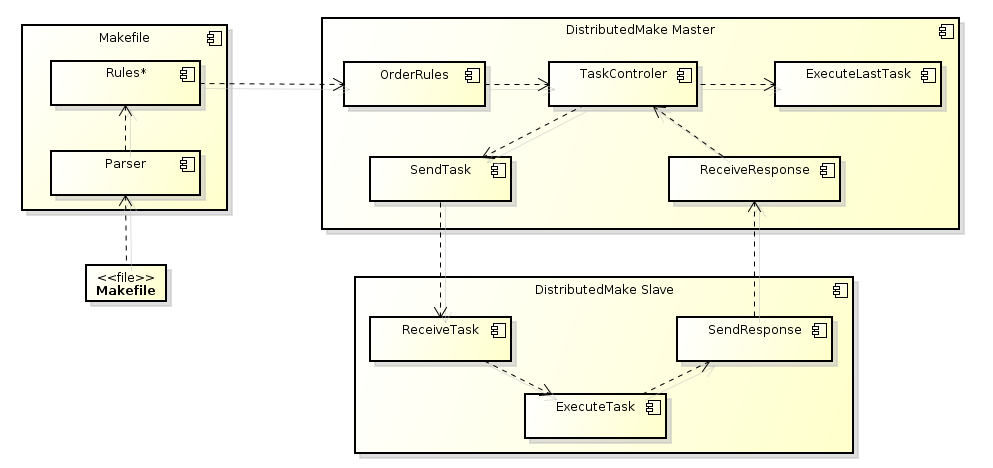
\includegraphics[scale=0.4]{schema.png}
  \caption{Architecture}
  \label{fig:architecture}
\end{figure}

\subsubsection{Rule}

Cette classe contient des informations telles que le nom de la cible
associée, sa liste de dépendances et sa liste de commandes à
exécuter. Elle contient aussi des méthodes pour vérifier si la cible
est un fichier (c'est à dire s'il existe un fichier de même nom et
qu'aucune de ses dépendances de type fichier n'a été modifiée
ultérieurement), pour vérifier l'heure de sa dernière modification ou
si elle a le bit exécutable.

\subsubsection{Makefile}

Cette classe est chargée de la lecture et du parsing d'un fichier
Makefile ainsi que du stockage de ses cibles et de son graphe des dépendances.

\subsubsection{DistributedMake}

C'est la classe principale du programme. Une instance de cette classe
peut être un maître ou un esclave, selon la façon dont il est créée
dans le programme. Indépendamment du rôle qu'elle joue, elle doit
recevoir un paramètre indiquant l'ID de son processus et le nombre
total de processus en cours. Ces informations sont récupérées à partir
d'un appel MPI. 

\paragraph{Maître}

Une fois initialisé, le maître crée un tableau des états des
processus esclaves et entre dans une boucle. Pour chaque processus
inactif, il envoie une règle avec ses commandes et ses dépendances et
le marque comme étant occupé. Quand un processus esclave indique qu'il a terminé la tâche,
le maître le marque comme étant capable d'en recevoir de nouvelles.

\paragraph{Esclaves}

Ces processus sont exécutés dans une boucle en attendant d'être assignés
à une tâche. Quand un esclave reçoit une tâche, il l'exécute et
renvoie les résultats (c'est à dire les fichiers générés) au maître.

\subsection{Protocole de communication}

\paragraph{Envoi des tâches}
Le protocole d'envoi d'une tâche comprend l'envoi de plusieurs
messages du maître vers l'esclave correspondant. Ces messages sont:
\begin{itemize}
\item \texttt{NB\_FICHIERS} : un entier avec le nombre de fichiers qui seront envoyés. Cette valeur inclut les dépendances et les fichiers exécutables contenus dans les commandes de la cible.
\item \texttt{FILE\_INFO} : pour chaque fichier, deux entiers en représentent la taille  (en octets) et le type (exécutable ou non). Si le fichier est exécutable, le processus esclave doit faire un \emph{chmod +x} lorsqu'il le reçoit.
\item \texttt{FICHIER} : une chaîne de caractères contenant le nom du
  fichier dans la première ligne et le contenu du fichier dans les lignes suivantes.
\item \texttt{NB\_COMMANDES} : un entier avec le nombre de commandes qui seront envoyées.
\item \texttt{COMMANDES} : ce message contient une chaîne de
  caractères comprenant toutes les commandes séparées par un
  \texttt{\\n}. Nous considérons que la taille maximale de chaque
  commande est de 2048 octets. 
\end{itemize}

Soit \texttt{$N$} le nombre de fichiers à envoyer, \texttt{$T_f$} la
taille du fichier le plus gros, \texttt{$C$} le nombre de commandes et
\texttt{$T_c$} la taille de la plus grande commande. Alors le nombre
total de messages à envoyer à un esclave est \texttt{$O(2 + 2 \cdot N
  + C)$} = \texttt{$O(N + C)$}. En supposant que la taille d'un entier
est de 4 octets, le nombre total d'octets envoyés à chaque tâche est
\texttt{$O(8 + N \cdot (T_f+8) + C \cdot T_c)$} = \texttt{$O(N \cdot
  T_f + C \cdot T_c)$}. 

\paragraph{Envoi des réponses}
Le protocole d'envoi d'une réponse est plus simple que celui d'envoi
d'une tâche. L'esclave n'envoie que les fichier générés par
l'exécution des commandes de la cible. Les messages sont donc
\texttt{NB\_FICHIERS} et pour chaque fichier \texttt{FILE\_INFO} et
\texttt{FICHIER}. La description de chaque message est la même que
celle faite pour l'envoi des tâches. 

L'analyse est similaire à l'envoi des tâches : soit \texttt{$N$} le
nombre de fichiers à envoyer et \texttt{$T_f$} la taille du fichier le
plus gros. Alors le nombre total de messages envoyés est \texttt{$O(1
  + 2 \cdot N)$} = \texttt{$O(N)$}. Le nombre total d'octets envoyés
est \texttt{$O(4 + N \cdot (T_f+8))$} = \texttt{$O(N \cdot T_f + C
  \cdot T_c)$}. 

\subsection{Installation}

La compilation de \emph{dmake} nécessite d'avoir une implémentation de
\emph{MPI} installée sur le système.
Les tests ont été effectués avec \emph{OpenMPI}. Pour l'installer, il
suffit d'exécuter la commande suivante :
\begin{verbatim}
> sudo apt-get install openmpi-dev
> sudo apt-get install openmpi-bin
\end{verbatim}

Pour compiler \emph{dmake}, il faut ensuite se placer à la racine du
répertoire \texttt{dmake/} puis exécuter la commande :
\begin{verbatim}
> make
\end{verbatim}

\subsection{Déploiement}

Pour déployer \emph{dmake}, il faut d'abord générer la liste des
machines sur lesquelles on souhaite déployer. Pour cela on utilise le
script python \texttt{createMachines.py} en ayant préalablement indiqué
les valeurs souhaitées pour les variables \texttt{startMachine},
\texttt{NUM\_MACHINES}, et \texttt{LAST\_MACHINE} : 
\begin{verbatim}
> python createMachines.py
\end{verbatim}

Ensuite le déploiement lui-même s'effectue à l'aide de
\texttt{mpirun}. Par exemple, pour lancer \emph{dmake} sur l'un des
exemples fournis dans l'archive, il faut se placer de le dossier
contenant l'exemple puis lancer la commande :
\begin{verbatim}
> mpirun -np NB_CORES -machinefile machines.txt PATH_TO_DMAKE
\end{verbatim}

\section{Tests de performances}

Les performances de \emph{dmake} ont été évaluées à l'aide d'un
benchmark programmé en C++.

\subsection{Méthodologie}

\paragraph{Configuration}
Le benchmark utilise un fichier de configuration
\texttt{benchmark.cfg} dans lequel on précise : 
\begin{itemize}
\item le nombre de fois
\texttt{NUM\_TIMES} qu'est répétée chaque exécution
\item  le nombre minimum \texttt{MIN\_MACHINES}
et le nombre maximum \texttt{MAXIMUM\_MACHINE} de de machines 
sur lesquel on souhaite exécuter les benchmarks
\item le pas \texttt{STEP} concernant le nombre de machines utilisées
  pour l'exécution
\item le type de test \texttt{MAKE\_TYPE} à exécuter. Peut avoit trois valeurs :
	\begin{itemize}
	\item  0 : On n'exécute que le dmake.
	\item  1 : On n'exécute que le make.
	\item  2 : On exécute make et dmake.
	\end{itemize}
\item la localisation \texttt{PATH\_TO\_DMAKE} de \emph{dmake}
par rapport à des tests qui seront exécutés
\item le répertoire \texttt{BASE\_FOLDER} oú se trouvent les tests
\item le nombre de tests à exécuter \texttt{NUM\_BENCHMARKS}
\item la liste des répertoires des tests \texttt{BENCHMARK1}, \texttt{BENCHMARK2}\dots
\end{itemize}

\begin{verbatim}
numTimes NUM_TIMES
machines MIN_MACHINES MAX_MACHINES
step STEP
make MAKE_TYPE
dmakeFolder PATH_TO_DMAKE
baseFolder BASE_FOLDER
numBenchmarks NUM_BENCHMARKS
BENCHMARK1
BENCHMARK2
...
\end{verbatim}

\paragraph{Fonctionnement}

Le programme \emph{benchmark} fonctionne de la manière suivante : pour
chaque fichier test proposé, il exécute successivement \emph{dmake} sur un nombre de
machines allant de \texttt{MIN\_MACHINES} à \texttt{MAX\_MACHINES}
qui est incrémenté de \texttt{STEP} machines à chaque tour. Pour un
fichier de test et un nombre de machines donnés, l'exécution est
répétée \texttt{NUM\_TIMES} fois afin d'obtenir un temps d'exécution moyen
qui soit représentatif. 
Pour chaque fichier test, le temps d'exécution moyen en fonction du
nombre de machines est écrit dans un fichier. Ce fichier est ensuite
utilisé par gnuplot pour générer la courbe correspondante. À cette
courbe est ajoutée une droite horizontale représentant le temps
d'exécution de \emph{GNU make} pour le fichier test considéré. 

\subsection{Conditions expérimentales}

Les test ont été effectués en salle D200. La salle était peu occupée
(environ 6 à 10 personnes). Cependant, les tests n'ayant pas tous été
effectués le même jour, les conditions expérimentales ont pu
varier. La charge du réseau notamment a pu être différente selon les
fichiers tests. Les makefiles utilisés pour les tests sont ceux
fournis par le professeur. Ils ont cependant subi les modifications
suivantes : 
\begin{itemize}
\item l'appel à des exécutables présents dans le répertoire courant est
  précédé d'un "./".
\item les fichiers nécessaires à l'exécution d'une cible ont été
  ajoutés dans les dépendances de celle-ci.
\item une cible "clean" a été ajoutée pour faire le nettoyage entre deux exécutions.
\end{itemize}

\paragraph{Environnement d'exécution}
\begin{description}
\item[Processeur :] 2 coeurs Intel Pentium D CPU 2.80GHz
\item[Mémoire :] 1Go
\item[OS :] ubuntu 11.04
\item[MPI :] OpenMPI 1.4
\item[Nombre d’ordinateurs :] 26
\end{description}

\subsection{Résultats et analyse}

Dans les graphiques suivants, le nombre de machines sur lesquelles est
lancée l'exécution est indiqué en abscisse, tandis que le temps
d'exécution en secondes ou l'accélération comparativement à une
exécution de \emph{GNU make} est indiqué en ordonnées.

Le benchmark a été réalisé sur un ensemble de 2 à 26 machines avec un pas de 3 machines. Chaque
exécution a été répétée 3 fois pour obtenir une moyenne
représentative.


\subsubsection{Blender 2.49}


\begin{figure}[h]
  \centering
  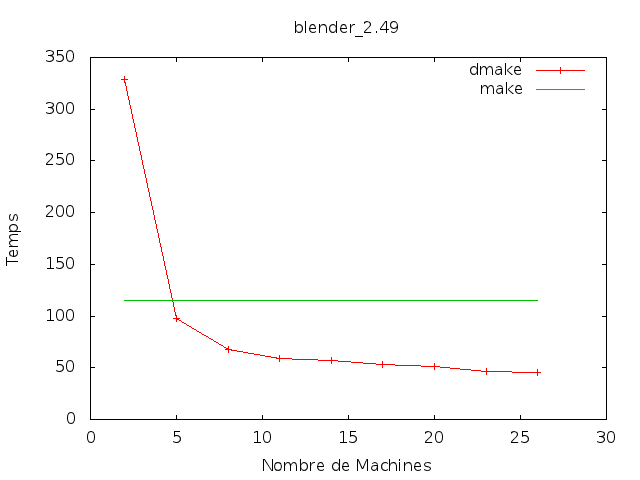
\includegraphics[scale=0.5]{graph_blender_2_49.png}
  \caption{Blender 2.49}
  \label{fig:blender249}
\end{figure}

On voit ici que l'expérimentation est conforme à nos attentes, car \emph{dmake} est plus rapide que \emph{GNU make} à  partir de cinq machines (cf. figure \ref{fig:blender249}). Le décalage par rapport à l'accélération idéale (cf. figure \ref{fig:blender249acc}) peut
être imputé à la partie du code qui est non parallèle ainsi qu'au communications sur le réseau. 

\begin{figure}[h]
  \centering
  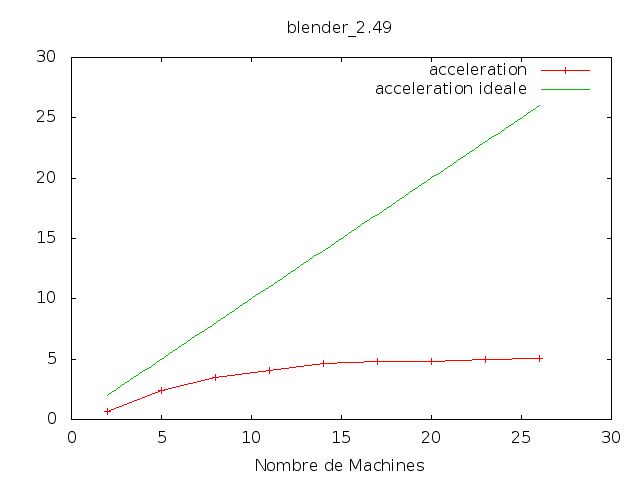
\includegraphics[scale=0.5]{acceleration_blender_2_49.png}
  \caption{Blender 2.49 : Accélération}
  \label{fig:blender249acc}
\end{figure}


\subsubsection{Premier}


\begin{figure}[h]
  \centering
  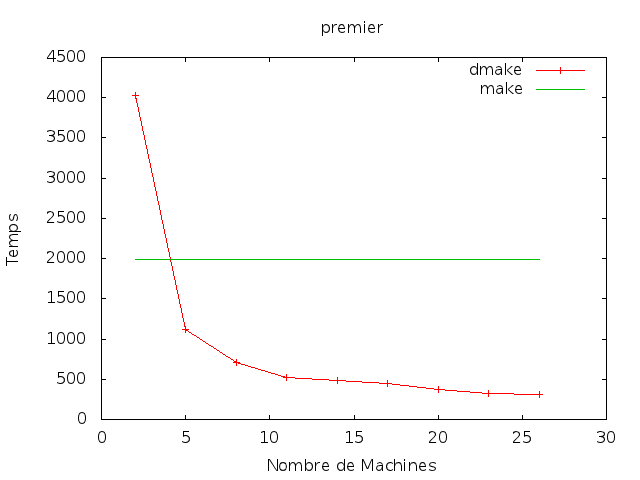
\includegraphics[scale=0.5]{graph_premier.png}
  \caption{Premier}
  \label{fig:premier}
\end{figure}

De même que précédemment, l'expérimentation est conforme à nos attentes, 
car \emph{dmake} est plus rapide que \emph{GNU make} à  partir de cinq machines (cf. figure \ref{fig:premier}). Le décalage par rapport à l'accélération idéale (cf. figure \ref{fig:premierAcc}) peut
être imputé à la partie du code qui est non parallèle ainsi qu'au communications sur le réseau. 
On constate que l'accélération est meilleure pour \emph{premier} que pour \emph{blender}. Cela peut s'expliquer par le fait que le temps d'exécution des tâches de \emph{premier} est proportionnellement plus grand que celui de  \emph{blender} par rapport au temps de communication.

\begin{figure}[h]
  \centering
  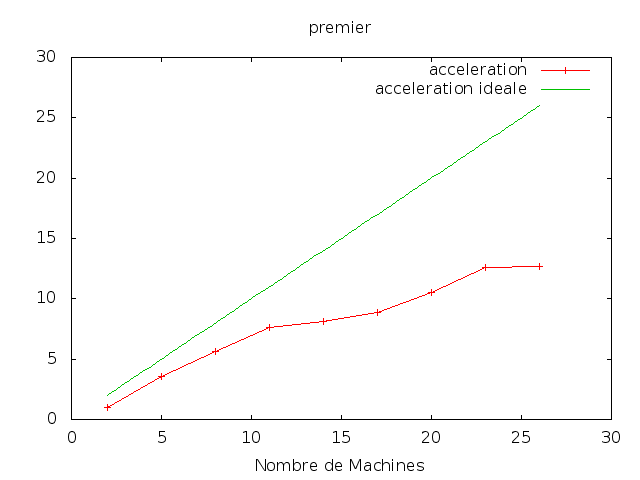
\includegraphics[scale=0.5]{acceleration_premier.png}
  \caption{Premier : Accélération}
  \label{fig:premierAcc}
\end{figure}

\subsubsection{Matrix}

\begin{figure}[h]
  \centering
  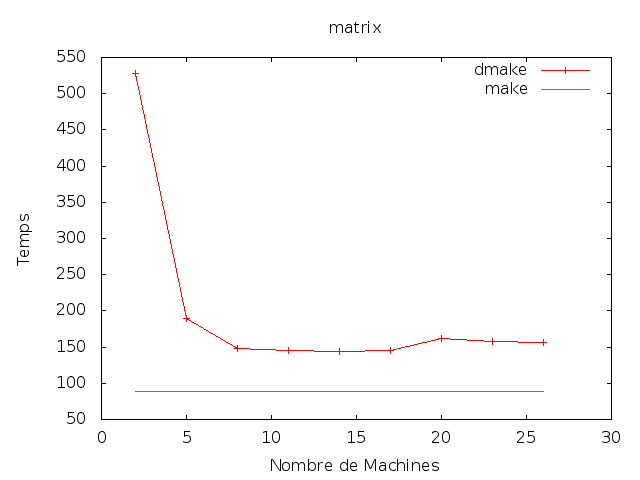
\includegraphics[scale=0.5]{graph_matrix.png}
  \caption{Matrix}
  \label{fig:matrix}
\end{figure}

On voit ici que l'expérimentation est contraire à nos
attentes. \emph{Dmake} est systématiquement plus lent que \emph{make},
même lorsque l'exécution est lancée sur un grand nombre de
machines (cf. figure \ref{fig:matrix}). Cela s'explique par le fait que ce test génère un très grand
nombre de fichiers de petite taille. Le temps de transfert de ces
fichiers entre les noeuds devient alors important par rapport au
temps d'exécution des tâches.

\begin{figure}[h]
  \centering
  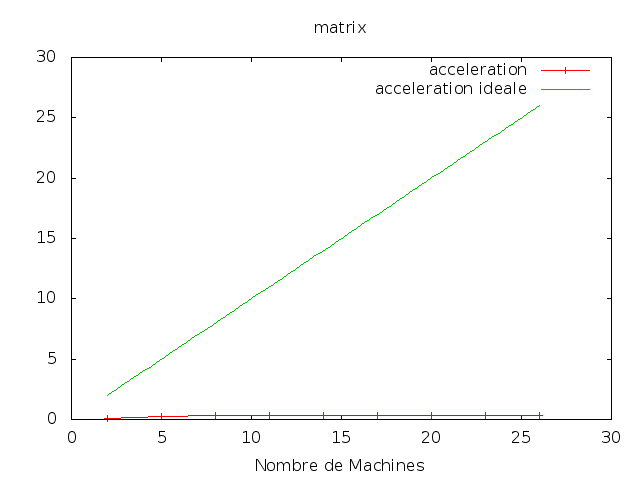
\includegraphics[scale=0.5]{acceleration_matrix.png}
  \caption{Matrix : Accélération}
  \label{fig:matrixAcc}
\end{figure}

\section*{Conclusion}
On constate que \emph{dmake} est efficace pour des makefiles dont les
tâches sont longues et relativement indépendantes
(cf. \texttt{premier}). En revanche lorsque le temps de communication
n'est plus négligeable devant le temps d'exécution des tâches, les
performances s'effondrent (cf. \texttt{matrix}). On constate le même phénomène lorsque les
tâches sont très dépendantes, car on s'approche alors d'une exécution séquentielle.

\subsection*{Passage à l'échelle}
Notre application peut traiter bien des tâches indépendantes et de traitement lourde. Les difficultés de passage à l'échelle arrivent quand nous avons des tâches très rapides qui exigent de nombreux transferts de fichiers (comme l'exemple "matrix"). Puisque notre ordonnancement des tâches se fait de manière centralisée, ce genre d'entrée (des tâches à grain fin) peut surcharger le maître et conduire à des résultats pas si bons. Par contre, avec une approche centralisée, nous avons une vue globale de l'état du système, donc on peut mieux gérer les dépendances pour prendre des décisions, ce qui augmente l'efficacité.

\end{document}
